\chapter{Introduction}

Online social networks have exploded into the lives of millions of people worldwide over the last decade, and their use has facilitated the interconnection of the world in ways never before perceived possible.

These social networks have many characteristics that are also exhibited by `real'-world social networks. Although most such platforms provide a different service to collaboratively satisfy an array of different use-cases, they tend to all be based around the idea of `friendships' (i.e. links between the user nodes in the social graph) and the sharing of information amongst friends.

Social networks like these have been available for around ten years now (with MySpace\footnote{http://myspace.com} launching in 2003 and Bebo\footnote{http://bebo.com} in 2005), but it wasn't really until the worldwide launch of Facebook\footnote{http://facebook.com} in 2006 that social networks became the staple, ubiquitous norm that they are today. More recently, we have seen the introductions of Google's social network grown from its Buzz service, Google Plus\footnote{http://plus.google.com}, Pinterest\footnote{http://pinterest.com}, App.net\footnote{http://app.net}, and many more. They make up a large part of and contribute heavily towards the ideas behind Web 2.0, which describes the web as being primarily formed from user-generated content and encourages the sharing of such content.

Another component that helped in the dawn of Web 2.0 was the rise of \textit{blogging}. A blog (`web-log') is a time-based series of posts consisting of continuous pieces of text, photos, or other media, and is generally contributed to by a single author. Blogs are often based around one or a set of topics and are usually public - meaning that they are written with the intention of being read by others. Despite this, they are often a way in which the author can look back at their history of posts, acting more as a diary recording snapshots of the author's life. Various blogging services exist on the web today, such as Medium\footnote{http://medium.com}, Wordpress\footnote{http://wordpress.com}, and Tumblr\footnote{http://tumblr.com}.


\section{Twitter as a Social Network}
Twitter\footnote{http://twitter.com} is an online social network, which launched in the summer of 2006 \cite{krishnamurthy08}. Since then, it has rapidly gained in popularity amongst several different user groups - teens and young people, casual users, celebrities, reporters, and so on - and within eight months had around 94,000 registered users \cite{java07}. Whilst the design of the site and its apps has changed significantly since its launch (Figures \ref{fig:old_twitter-new_twitter}(\subref{fig:old_twitter}) and \ref{fig:old_twitter-new_twitter}(\subref{fig:new_twitter})), its function has remained mostly constant. Twitter has never been a direct competitor with Facebook, as users tend to use the two sites concurrently for different purposes: whilst Facebook's focus is on providing many services at once (such as photo-sharing, commenting/endorsing of information, messaging, pages for businesses, groups, events, etc.), Twitter's is more on simplicity.

\begin{figure}[h]
\begin{subfigure}{.9\textwidth}
    \centering
    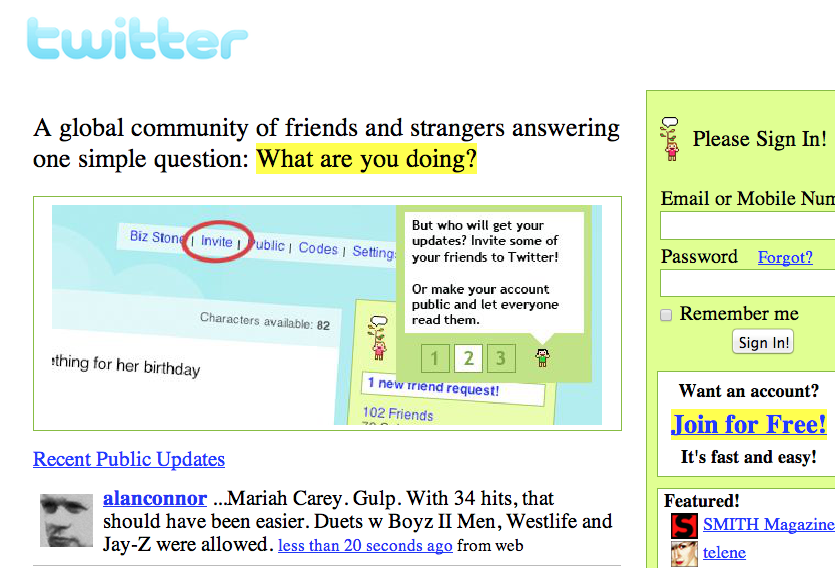
\includegraphics[scale=0.4]{1.Introduction/Media/old_twitter.png} 
    \caption{Twitter's landing page in 2006.}
    \label{fig:old_twitter}
\end{subfigure}\\
\begin{subfigure}{.9\textwidth}
    \centering
    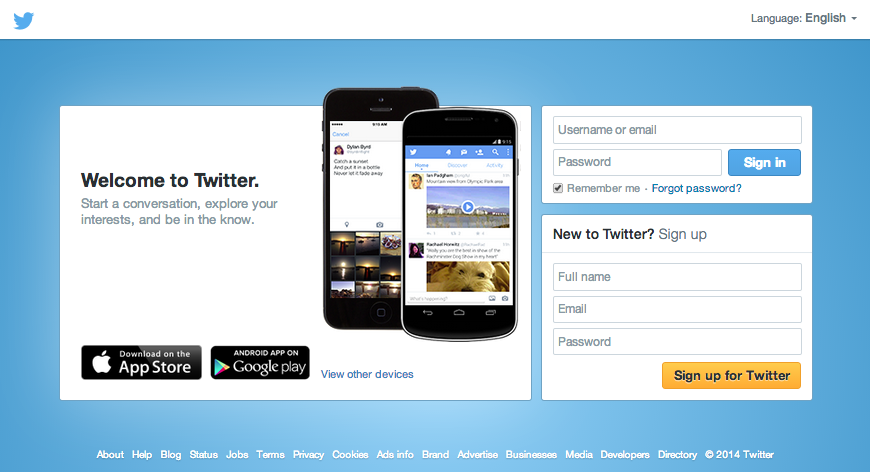
\includegraphics[scale=0.4]{1.Introduction/Media/new_twitter.png} 
    \caption{Twitter's landing page in 2014.}
    \label{fig:new_twitter}
\end{subfigure}
\caption{Twitter's 2006 homepage (from http://web.archive.org) compared to its 2014 homepage}
\label{fig:old_twitter-new_twitter}
\end{figure}


More specifically than just being an online social network, Twitter is a microblogging website. Whilst a blog, as mentioned, typically contains long posts, Twitter only allows its users to post short pieces of text, up to 140 characters in length \cite{krishnamurthy08, huberman08}, called `Tweets'. Thus, Twitter is a hybrid social network and blogging service and whilst each Tweet may only realistically be able to hold a couple of sentences, this system facilitates quick, timely, and `real-time' \textit{live} information-sharing amongst its millions of users \cite{zhao09}. Its idea is that short pieces of news will `travel' faster and will be seen by more people more quickly than traditional news stories.

Although Tweets are limited to 140 characters in length, the inclusion of URLs is allowed. This enables further extension of Tweets through external websites, and supports the inclusion of links to images and videos. Twitter has encouraged this use-case by providing `share' buttons for developers to embed in websites, and direct support for photo and video applications, such as TwitPic\footnote{http://twitpic.com} and Vine\footnote{http://vine.com}.

Its simplicity has also helped its growth into the mobile domain, in which smartphone users are able to very quickly post updates about their lives, a piece of information they want to share, or a photo or video, and be able to post it \textit{as it happens} directly from the news source or geographical location \cite{castillo11}. This has been especially useful in emergency situations worldwide, including the Haiti earthquake in 2010 \cite{muralidharan11}, and 2011's Egyptian protests \cite{wilson11} and Thai flood \cite{kongthon12}. Indeed, \citet{sakaki10} used Twitter to build an earthquake-reporting system for Japan that outperforms the Japan Meteorological Agency in terms of its promptness of notification.

Use of Twitter is based around `timelines' of Tweets, to which new Tweets are pre-pended as they are posted by users. The \textit{home} timeline is the default view, in which Tweets from all of a person's subscribed-to users are placed. Timelines of an individual user contain only Tweets from that user, and are known as a `user' timeline. Customisation of timelines is also possible through the use of Twitter lists, in which different users can be placed to categorise streams of Tweets from different sets of users.


\section{The Social Graph and Information Flow}
The structure of Twitter lies within the users and their connectivity within its social graph. However, unlike Facebook, whose social structure is made up of bi-directional `friendships' between users, Twitter's primary social graph is made up more of mono-directional links between its users \cite{edwards13}. A person using Twitter can elect to \textit{follow} another user, which subscribes the person to receive all of that user's Tweets to their home timeline. The set of users that follow a person are known as that person's \textit{followers}, and the set of users that the person follows are the person's \textit{friends}. Therefore, if two users both mutually follow each other, then the link between them is bi-directional.

Whilst bi-directional links are common amongst communities of similar interests, friends, colleagues, and so on, mono-directional links are found more in situations in which less-influential users follow more-influential users, such as celebrities.


\section{The Problem}
\label{section:research_questions}
A person who follows a set of other users can generally be assumed to find them to produce more interesting information than those that the person does not follow. However, despite that, not \textit{all} information produced by a followed user is likely to be interesting to the person, and yet \textit{all} information produced by a Twitter friend will be received onto the home timeline.

Noise is a common problem in Twitter, and is the uninteresting information one might receive that conveys little interest. It is likely that most of the information received on Twitter \textit{is} uninteresting \cite{alonso10}, and this makes it very hard to distinguish the interesting from the uninteresting.

Since people tend to use Twitter most in short and sporadic moments, looking for a quick news or information fix, they do not have time to filter out noisy Tweets. Thus, the presence of noise can dampen the user's experience, making it much more difficult to find the interesting information.

In addition, Twitter users typically exist within an information `bubble'. This is similar to the notion of the Google search bubble, in which the search engine uses previous results and search terms to only return information to a user based on what \textit{it thinks} the user would find the most interesting and useful. This results in the users not knowing which information exists beyond the confines of their bubble, and if they do not know it exists, they cannot know if it is of interest to them. Similarly, a Twitter user cannot follow all of the users he/she may find interesting, since he/she will not \textit{know} of all the interesting users existing on the social graph.

Although not directly answered in this research, the key theme and motivation behind the work it involves is;\\
\centerline{\textbf{How can users be exposed to \textit{interesting} and \textit{relevant} information,}}
\centerline{\textbf{but without explicit subscription or search?}}

The remaining chapters aim to go some way to answering this question through a focus on understanding information propagation, and how combining this with knowledge of the social structure of Twitter can assist towards solving the problem of identifying interesting and relevant information and determining it from the noise surrounding it. Whilst other work in the area, discussed further in the Background chapter, has also researched into the notions of relevance and interest in online social networks, and Twitter in particular, they do not address the problem in the same way or attempt to validate findings so thoroughly.

The central thesis addressed by this research is that the interestingness of Tweets in Twitter can be non-semantically inferred through consideration of the underlying social graph model and the use of humans as proxies to the perception of interesting information. In this work, the following research questions help illustrate the steps towards realising this thesis: 
\begin{itemize}
    \item \textbf{RQ1} \textit{Does Tweet popularity, measured in terms of retweets, \textbf{define} interesting information?}
    \item \textbf{RQ2} \textit{Can Tweet popularity, measured in terms of retweets, \textbf{be an indicator} of interesting information?}
    \item \textbf{RQ3} \textit{Is the arrangement of Twitter's social graph an important factor in retweet propagation, and thus perceived popularity?}
    \item \textbf{RQ4} \textit{Can Tweet interestingness be inferred \textbf{non-semantically}?}
\end{itemize} 

In answering these questions, the main contributions made in this research work are outlined below.
\begin{itemize}
    \item Tweet analysis allows for providing definitions for key concepts, such as retweet groups and propagation path-length, to form foundations for further definitions and work towards substantiating the thesis.
    \item Social graph analysis shows how the underlying edges dictate information flow through Twitter, and that altering the network structure has a clear effect on the propagation characteristics of Tweets within it.
    \item A mathematical `definition' of global interestingness is provided, given as a score for the purposes of quantifying and ranking Tweets by this metric. The score is an estimation based from a Tweet's predicted popularity.
    \item Rigorous validation tests are conducted to demonstrate the score's ability to identify useful Tweets from noise and rank information by interestingness. User tests involving Tweets `local' to them on the social graph show that there is scope for the scores to also be applied locally as well as globally (for addressing information relevance). 
\end{itemize}


\section{Thesis Structure}
The chapters containing the remainder of this thesis are laid out as follows.

\begin{itemize}
    \item \textbf{Background and Research Domain} - A chapter providing an introduction to key concepts and the ideas behind the main research. Also included is a review of relevant literature across the range of topics addressed in the thesis.
    \item \textbf{Understanding the Behaviour of Retweeting on Twitter} - Initial research into the problem areas identified, including studies into the propagation characteristics exhibited by Twitter and its useful and interesting properties. This is in order to provide an understanding of the mechanics of retweets.
    \item \textbf{Analysis of Twitter's Social Structure} - An in-depth analysis into the layout of Twitter's social graph and the ways in which it helps govern the potential spread of retweets. From this graph analysis, an initial method for inferring Tweet interestingness emerges.
    \item \textbf{Inferring Interestingness} - Improvements to the inference methodology are introduced, and deeper validations and analyses are conducted into the relative strengths of the new method. Different types of assessments are conducted in order to investigate the performance on a general scale as well as moving towards addressing information relevance.
    \item \textbf{Assessment and Conclusions} - The thesis ends with a general analysis and conclusion, and a discussion of potential future work in this area and leading on from this research. The contributions are summarised and the research questions answered more formally.
\end{itemize}
